

\documentclass[12pt,oneside]{article}

%%%%%%%%%%%%%%%%%%%%%%%%%%%%
%%   Zusaetzliche Pakete  %%
%%%%%%%%%%%%%%%%%%%%%%%%%%%%
\usepackage{enumerate}  
\usepackage{fancyhdr}
\usepackage{a4wide}
\usepackage[utf8]{inputenc}
\usepackage{graphicx}
\usepackage{palatino}
\usepackage{multirow}
\usepackage{booktabs}
\usepackage{titlesec}
\usepackage{amsthm}
\usepackage{amssymb}
\usepackage{amsmath}
\usepackage[utf8]{inputenc}
\usepackage[options ]{algorithm2e}
\usepackage[ruled,vlined]{algorithm2e}
\usepackage{lmodern}
\usepackage[utf8]{inputenc}
\usepackage[english,german]{babel}
\usepackage{xcolor}
\usepackage{amsfonts}
\usepackage{etoolbox}
\usepackage[]{algorithm2e}
\usepackage{blindtext}
\usepackage{algorithm}
\usepackage[noend]{algpseudocode}
\usepackage{enumitem}% http://ctan.org/pkg/enumitem

% notendig für Definitionen und Theoreme
\newtheorem{theorem}{Theorem}[section]
\newtheorem{corollary}{Corollary}[theorem]
\newtheorem{lemma}[theorem]{Lemma}
\newtheorem{fact}[theorem]{Fakt}

\newtheorem{prop}{Proposition}[section]

\theoremstyle{remark}
\newtheorem*{remark}{Remark}

\theoremstyle{definition}
\newtheorem{definition}{Definition}[section]
%%%%%%%%%%%%%%%%%%%%%%%%%%%%%%

%folgende Zeile auskommentieren für englische Arbeiten
\usepackage[ngerman]{babel}
%folgende Zeile auskommentieren für deutsche Arbeiten
%\usepackage[ngerman, english]{babel}

\usepackage[T1]{fontenc}
\usepackage[utf8]{inputenc}
\usepackage[bookmarks]{hyperref}
\usepackage[justification=centering]{caption}
\usepackage[style=authoryear,natbib=true,backend=biber,maxbibnames=20]{biblatex}
\usepackage{csquotes}
\bibliography{literatur}

\setlength{\parindent}{0em} 
\setlist[itemize]{noitemsep, topsep=0pt}
\setlist[enumerate]{noitemsep, topsep=0pt}


%%%%%%%%%%%%%%%%%%%%%%%%%%%%%%
%% Definition der Kopfzeile %%
%%%%%%%%%%%%%%%%%%%%%%%%%%%%%%

\pagestyle{fancy}
\fancyhf{}
\cfoot{\thepage}
\setlength{\headheight}{16pt}

%%%%%%%%%%%%%%%%%%%%%%%%%%%%%%%%%%%%%%%%%%%%%%%%%%%%%
%%  Definition des Deckblattes und der Titelseite  %%
%%%%%%%%%%%%%%%%%%%%%%%%%%%%%%%%%%%%%%%%%%%%%%%%%%%%%

\newcommand{\JMUTitle}[9]{

  \thispagestyle{empty}
  \vspace*{\stretch{1}}
  {\parindent0cm
  \rule{\linewidth}{.7ex}}
  \begin{flushright}
    \vspace*{\stretch{1}}
    \sffamily\bfseries\Huge
    #1\\
    \vspace*{\stretch{1}}
    \sffamily\bfseries\large
    #2\\
    \vspace*{\stretch{1}}
    \sffamily\bfseries\small
    #3
  \end{flushright}
  \rule{\linewidth}{.7ex}

  \vspace*{\stretch{1}}
  \begin{center}
    
\includegraphics[width=4in]{logo} \\
    \vspace*{\stretch{1}}
    \Large  Bachelorarbeit   \\

    \vspace*{\stretch{2}}
   \large Lehrstuhl für Mathematik \\
    \large und Informatik \\
    \large Universität Leipzig\\
    \vspace*{\stretch{1}}
    \large Betreuer:  #8 \\[1mm]
    
    \vspace*{\stretch{1}}
    \large Leipzig, den #7
  \end{center}
}

\titlespacing*{\section}
{0pt}{3.5ex plus 1ex minus .2ex}{.2ex plus .2ex}
\titlespacing*{\subsection}
{0pt}{1.5ex plus 1ex minus .2ex}{.2ex plus .2ex}
\titlespacing*{\subsubsection}
{0pt}{1.5ex plus 1ex minus .2ex}{.2ex plus .2ex}

%%%%%%%%%%%%%%%%%%%%%%%%%%%%
%%  Beginn des Dokuments  %%
%%%%%%%%%%%%%%%%%%%%%%%%%%%%

\begin{document}

  \JMUTitle
      {Komplexität und Evaluation des AKS-Primzahltests  }  
      {Salman Salman}                        
      {3753924}
      
      {Fakultät für Informatik und Mathematik}  % Name der Fakultaet
      {Leipzig 2020}                          % Ort und Jahr der Erstellung
      {\today}                              % Tag der Abgabe
      {Prof. Dr. Andreas Maletti}               % Name des Erstgutachters
      {Zweitgutachter}                          % Name des Zweitgutachters
      
  \clearpage

\lhead{}
\pagenumbering{Roman} 
    \setcounter{page}{1}

\tableofcontents
\clearpage

\addcontentsline{toc}{section}{\listfigurename}
\listoffigures

\addcontentsline{toc}{section}{\listtablename}
\listoftables
\clearpage

\setlength{\parskip}{0.5em} 


%%%%%%%%%%%%%%%%%%%%%%%%%%%%
%%  Kurzzusammenfassung   %%
%%%%%%%%%%%%%%%%%%%%%%%%%%%%
\lhead{Abstract}
\section*{Abstract}
Primzahlen haben in der Informatik, speziell im Anwendungsgebiet der Kryptographie, eine sehr hohe Relevanz für moderne kryptographische Systeme ist es von Wichtigkeit selbige schnell bestimmen zu können. Hierzu werden effiziente Algorithmen zur Lösung des mathematischen Primalitätsproblem benötigt. Das Primalitätsproblem umfasst die Frage um die Entscheidung, ob eine gegebene Zahl eine Primzahl ist oder nicht. Der erste deterministische Primzahltest in Polynomialzeit wurde von den indischen Informatikern Agrawal, Kayal, und Saxena vorgestellt. Der nach ihnen benannte AKS-Algorithmus wird im Rahmen dieser Arbeit repräsentiert, implementiert und evaluiert. Außerdem wird die Korrektheit des Algorithmus experimentell geprüft und mathematisch bewiesen. 


%%%%%%%%%%%%%%%%%%%%%%%%%%%%
%%  Einstellungen  %%
%%%%%%%%%%%%%%%%%%%%%%%%%%%%
\clearpage
\pagenumbering{arabic}  
    \setcounter{page}{1}
\lhead{\nouppercase{\leftmark}}

%%%%%%%%%%%%%%%%%%%%%%%%%%%%
%%  Hauptteil  %%
%%%%%%%%%%%%%%%%%%%%%%%%%%%%

 

\section{Einleitung} \label{einleitung}

\subsection{Gliederung der Arbeit}
Die Arbeit gliedert sich in vier Bestandteile, wobei der
erste Teil die Einleitung darstellt. Dort wird ein kurzer Überblick in das Thema gegeben und die Zielsetzung der Arbeit definiert.

Das zweite Kapitel enthält die Grundlagen und die Definitionen. Hier werden Terminologie und Konzepte erläutert, die für das weitere Verständnis der Arbeit eine Rolle spielen. 

Der Algorithmus und seine Korrektheit sind die Bestandteile des dritten Kapitels. Zuerst wird die Grundidee des Algorithmus erläutert, danach wird der Algorithmus in seiner ursprünglichen Form(wie im AKS-Paper) angegeben. Anschließend wird der Korrektheitsbeweis des Algorithmus geführt.

Im vierten Kapitel wird die Laufzeitanalyse des Algorithmus vorgestellt, dabei werden die Laufzeit der einzelnen Schritte (STEPS 1-6) des Algorithmus ausführlich analysiert.    

\subsection{Überblick}
Eine Primzahl ist eine von 1 verschiedene natürliche Zahl, die keine Teiler außer 1 und sich selbst hat. Die Frage, ob eine Zahl eine Primzahl ist oder nicht, war schon im antiken Griechenland interessant. Euklid hat sich mit dieser Frage beschäftigt und beweisen, dass es unendlich viele Primzahlen gibt. Im 3. Jahrhundert v. Chr. hat der griechische Mathematiker Eratosthenes einen Algorithmus zur Bestimmung einer Liste aller Primzahlen kleiner oder gleich einer vorgegebenen Zahl vorgestellt, dieser Algorithmus ist jedoch zur Lösung des Primalitätsproblem nicht effizient, da die Generierung solcher Listen bei sehr großen Zahl zu aufwendig wird. Im 17. und 18. Jahrhundert haben Wissenschaftler versucht eine Formel für Primzahlen zu erfinden. Der französische Wissenschaftler Marin Mersenne hat eine Formel für die nach ihm sogenannten Mersenne-Zahlen entwickelt, 51 der bekannten Mersenne-Zahlen sind Primzahlen. Solche Zahlen heißen Mersenne-Primzahlen, die größte Primzahl heute $2^{82,589,933} − 1$ ist eine Mersenne-Primzahl. Ein anderer französischer Mathematiker Pierre de Fermat hat einen Satz zur Beschreibung der Eigenschaften von Primzahlen, aufgestellt. Auf seinen Satz bauen viele Primzahltests(einschließlich des AKS-Primzahltests) auf. \newline\newline
Im Laufe der Zeit wurden auch mehrere Algorithmen zur Lösung des Primalitätsproblems entwickelt, die entweder von unbewiesenen Hypothesen, wie zum Beispiel die verallgemeinerte Riemannsche Vermutung abhängig waren oder probabilistisch waren. Probabilistische Algorithmen sind randomisierte Algorithmen, die auch ein falsches Ergebnis liefern können. Ein bekannter probabilistischer Primzahltest ist der Miller-Rabin-Primzahltest, er kann das Primalitätsproblem in $O(k log^3 n)$ lösen. Dennoch kann der beste nicht probabilistische Algorithmus (vor AKS) das Primalitätsproblem in $ \Omega(\sqrt{n}) $ Schritten lösen, wobei $n$ die Eingabegröße ist(Anzahl der nötigen Bits, um die Zahl $n$ zu repräsentieren). Solcher Algorithmus braucht exponentielle Zeit, um das Problem zu lösen. In 2002 haben drei Informatiker Agrawal, Kayal, und Saxena den ersten deterministischen unbedingten Algorithmus entwickelt, der das Primalitätsproblem in Polynomialzeit lösen kann. Das heißt sie haben gezeigt, dass das Primalitätsproblem(PRIMES) zur Komplexitätsklasse $P$ gehört.      

\subsection{Zielsetzung}
In dieser Arbeit wird der AKS-Primzahltest Algorithmus aus dem Orginalpaper behandelt. Ziel dieser Arbeit ist die Korrektheit des AKS-Algorithmus zu testen und evaluieren. Dabei wird die Idee Algorithmus dargestellt und erläutert, danach kommt die Analyse der Korrektheit, da wird die Korrektheit zuerst mathematisch bewiesen, dafür wird ein bidirektionaler Beweis geführt, wo gezeigt wird, dass wenn der Algorithmus PRIME liefert, ist die Zahl auch eine Primzahl. Aber auch wenn die Eingabe eine Primzahl ist, liefert der Algorithmus PRIME. Dazu wird seine Korrektheit auf einem Rechner implementiert und getestet. Der Algorithmus ist dafür bekannt, das Primalitätsproblem in Polynomialzeit zu lösen, diese Eigenschaft wird auch zuerst mathematisch bewiesen. Schließlich soll die Polynomialzeit Eigenschaft durch eine Grafik experimentell bewiesen.  

Um die Korrektheit zu demonstrieren, soll der Algorithmus in Python implementiert werden, dabei wird die Ausgabe des Algorithmus bei mehreren Zahlen(meistens große Zahlen) geprüft. Zudem soll auch die Laufzeit durch eine Grafik illustriert werden.  


\section{Definitionen und Grundlagen}
In diesem Kapitel werden die essenziellen Begriffe und Theoreme aus der Zahlentheorie, der Algebra und der Komplexitätstheorie, die für den AKS-Algorithmus relevant sind, definiert. In diesem Kapitel handelt es sich darum, einen formalen Literaturhinweis zu haben, um später die hier definierten Begriffe und Theoreme zu referenzieren.
% Definitionen der Zhalentheorie 
% Definitonen
\subsection{Zahlentheorie}
\theoremstyle{definition}
\begin{definition}\label{Df_1}
Seien $a,b \in \mathbb{N}$. Der \textbf{größte gemeinsame Teiler} von $a$ und $b$ wird mit $(a,b)$ bezeichnet, ist die größte positive Zahl $n$, sodass $n \mid a$ und $n$ $ \mid b$
\end{definition}

\smallskip 

\begin{definition}\label{Df_2}
Zwei Zahlen $a,b \in \mathbb{N}$ heißen genau dann \textbf{Teilerfremd}, wenn $(a,b) = 1$.
\end{definition}

\smallskip

\begin{definition}
Seien $n, m$ zwei natürliche Zahlen, dann heißt die kleinste positive natürliche Zahl, die sowohl ein Vielfaches von $n$, als auch von $m$ \textbf{kleinstes gemeinsames Vielfaches} beider zahlen. Hier wird das kleinste gemeinsame Vielfaches mit \textbf{kgV} bezeichnet.
\end{definition}

\smallskip 

\begin{definition}\label{Df_3}
Seien $a, b, n \in \mathbb{N}$. a ist genau dann \textbf{kongruent} zu $b$ modulo $n$, wenn $n \mid a - b $ gilt, dies wird mit $a = b$ (mod $n$) bezeichnet.  
\end{definition}

\smallskip 

\begin{definition}\label{Df_4}
Seien $r,n \in \mathbb{N}$ mit $(n,r) = 1$, dann ist die \textbf{Ordnung} von $n$ modulo $r$ das kleinste $k$, sodass $n^k = 1 (mod $ r). Die Ordnung wird mit $o_{r}(n)$ bezeichnet.
\end{definition}

\smallskip


\begin{definition}\label{Df_5}
Sei $n \in \mathbb{N}$, die \textbf{Primzahlzerlegung} von $n$ ist die Darstellung der Zahl als Produkt ihrer Primfaktoren \newline
\begin{equation}
    n = p_{1}^{e_{1}}p_{2}^{e_{2}}...p_{M}^{e_{M}}
\end{equation}
Wobei $e_{k}$ die Vielfachheit der Primzahl $p_{k}$ ist.
\end{definition}

\smallskip


\begin{definition}\label{Df_6}
Sei $n \in \mathbb{N}$ mit $n > 1$. Die \textbf{eulersche Phi-Funktion} wird mit $\phi(n)$ bezeichnet, ist die Anzahl der Zahlen $k, \, 1 \leq k \leq n$, sodass $(k,n) = 1$
\end{definition}

\smallskip


% Theoreme
\begin{theorem}[\textbf{Satz von Euler}]\label{Th_1}
Seien $a,n \in \mathbb{N}$ teilerfremd, \newline dann gilt $a^{\phi(n)} = 1 $(mod n).
\end{theorem}

\begin{proof}
    
Seien $R =\{ a \in \mathbb{N} \mid (a,n) = 1 \} =  \{a_{1}, a_{2},...,a_{\phi(n)} \}$ und $c \in R, c \leq n$.\newline\newline Da $(c,n) = (a_{i},n) = 1$, gilt auch $(c \cdot a_{i}, n) = 1$ \newline\newline und damit ist auch $a_{i} = c \cdot a_{j}$(mod $n$) wahr für ein $a_{j} \in R \Rightarrow a_{i} = a_{j}$. Das heißt es gilt:\newline
\begin{equation}
     \prod_{k = 0}^{\phi(n)} c \cdot a_{k} =
     c^{\phi(n)}\prod_{k = 0}^{\phi(n)} a_{k} = \prod_{k = 0}^{\phi(n)}  a_{k} (mod \, n )
\end{equation}
    
     $\Rightarrow c^{\phi(n)} = 1$ (mod $n$).

\end{proof}

\smallskip

\begin{theorem}[\textbf{Binomischer Lehrsatz}]\label{Th_3}
Seien R ein kommutativer Ring und n eine natürliche Zahl, dann gilt für $a,b \in $R:\newline\newline
 \begin{equation}
     (a + b)^n  = \sum_{k=0}^n {n \choose k} a^k b^{n-k}.
 \end{equation}
\end{theorem}

\smallskip

\begin{theorem}\label{th_25}
Sei n eine Primzahl, dann gilt ${n \choose i} = 0 $(mod n).
\end{theorem}

\begin{proof}
\begin{equation}\label{modb}
    {n \choose i} = \frac{(n - i - 1) \cdot \cdot \cdot (n - 1) \cdot n }{i!}
\end{equation}
Da $n$ im Zähler steht und n eine Primzahl ist(nicht durch Zahlen im Nenner teilbar), muss die obere Gleichung (\ref{modb}) durch n teilbar sein. 
\end{proof}

\smallskip

\begin{theorem}[\textbf{Kleiner Satz von Fermat}]\label{Th_2}
Für eine Primzahl $p$ und ein beliebiges $a \in \mathbb{Z}$ gilt:
\begin{align*}
    a^p = a \, mod \, p
\end{align*}
\end{theorem}

\begin{proof}
Die Aussage kann per Induktion über $a \in \mathbb{Z}_{+}$ gezeigt werden.\newline\newline
IA: $a = 0  \Rightarrow 0^p = 0 \, mod \, p$.\newline\newline

IH: Nun sei die Aussage für ein beliebiges $a \in \mathbb{Z}_{+}$ wahr.\newline\newline

IS: für a + 1 gilt nach dem binomischen Lehrsatz:
\begin{align*}
    (a + 1)^p - (a + 1) = \big{[}a^p + {p \choose 1}a^{p - 1} + ... +{p \choose p - 1} a + 1\big{]} - (a + 1).
\end{align*}
Für die Koeffizienten gilt: 
\begin{align*}
    {p \choose k} = \frac{p \cdot (p - 1) \cdot \cdot \cdot (p - k + 1)}{1 \cdot 2 \cdot \cdot \cdot k}
\end{align*}
$\forall k, \,  1 \leq k \leq p - 1$, somit sind alle Koeffizienten(bis auf das erste und das letzte) durch p teilbar.\newline\newline
Also es gilt:
\begin{align*}
(a + 1)^p - (a + 1) = \big{[} a^p + 1 \big{]} - (a + 1) = a^p - a \, mod \, p.
\end{align*}
und das ist nach der IH durch p teilbar.\newline  
\end{proof}

\smallskip

\begin{theorem}[\textbf{Gaußsche Summeformel}]\label{gauss}
Sei n eine natürlich Zahl, dann gilt:
\begin{equation}
    \sum_{i = 1}^{n} i = \frac{n (n + 1)}{2} = \frac{n^2 + n}{2} 
\end{equation}
Der Beweis ist durch Induktion trivial. 
\end{theorem}



% Algerba

\subsection{Algebra}
\textbf{Bemerkung:} In diesem Kapitel wird davon ausgegangen, dass die grundlegenden Definitionen von Gruppen, Ringen, Körpern und ihre Eigenschaften dem Leser bekannt sind. Hier werden Theoreme und Begriffe der Algebra und Polynomentheorie, die später für den Korrektheitsbeweis von Bedeutung sind, vorgestellt und bewiesen.\newline

\begin{definition}
Sei $R$ ein Ring, dann ist der \textbf{Polynomring} $R[X]$ die Menge aller Polynome der Form $a_{0} + a_{1}X + a_{2} X^2 + ... + a_{n}X^n$, wobei $a_{0},a_{1}...,a_{n} \in R$.
\end{definition}

\smallskip

\begin{definition}
Sei $f = (a_0, a_1,...a_n) \in R[X], \, f \neq 0 $ ein Polynom, dann heißt
\begin{align*}
    deg \, f = max \{ i  \mid a_i \neq 0 \}
\end{align*}
\end{definition}

\smallskip

\begin{definition}
Sei $I$ eine Teilmenge des Rings $(R,+,\cdot)$. $I$ heißt \textbf{Ideal}, wenn gilt:
\begin{enumerate}
    \item $0 \in I$.
    \item $\forall a,b \in I$ ist $a + b \in I$.
    \item $\forall a \in I$ und $r \in R$ ist $r \cdot a \in I$.
    \item $\forall a \in I$ und $r \in R$ ist $a \cdot r \in I$.
\end{enumerate}
\end{definition}

\smallskip 

\begin{definition}
ist $(R, +, \cdot)$ ein Ring und $I$ ein Ideal von R, dann bildet die Menge $R/I = \{ a + I \mid a \in R\}$ der Äquivalenzklassen modulo $I$ mit folgenden Verknüpfungen einen Ring:
\begin{itemize}
    \item $(a + I) + (b + I) = (a + b) + I$.
    \item $(a + I) \cdot (b + I) = (a \cdot b ) + I$.\newline
\end{itemize}
Diesen Ring nennt man den \textbf{Quotientenring}. 
\end{definition}

\smallskip

\begin{theorem}\label{number_of_roots}
Sei $R$ ein kommutativer Ring und $f \in R[X]$ ein Polynom, sodass $f \neq 0$. Ferner seien $a_1, a_2,...,a_n \in R$ die Nullstellen/Wurzeln von $f$ mit $a_i - a_j \in R^*, \, \forall i,j, \, 1 \leq i,j, \leq n$. Dann ist $deg \, f \geq n$.
\end{theorem}

\begin{proof}
Beweis durch Widerspruch, angenommen $deg \, f = n - 1$ für ein beliebiges $n$. Sei $f(X) = b_{n-1}X^{n-1} + b_{n-2}X^{n-2} + ... + b_1 X + b_0$ mit $b_{n-1} \neq 0$. Weiterhin seien $a_1,a_2,...,a_{n}$ die Wurzeln des Polynoms $f(X)$, dann gilt $f(a_i) = 0, \, \forall 1 \leq i \leq n$, das heißt $b_{n-1} a_i^{n-1} +...+ b_1 a_i + b_0 = 0, \, \forall 1 \leq i \leq n$. \newline\newline Zudem sei $A = [a_{i,j}]_{1 \leq i,j \leq n}$ die Matrix der Wurzeln und $b = (b_1 b_2 ...b_{n}) \neq 0$ der Vektor der Koeffizienten von $f(X)$. Dann gilt $b \cdot A = 0$, aber $det \, A \neq 0 \Rightarrow  b = 0$ und dies ist ein Widerspruch(Da $b \neq 0$), daraus folgt es existiert $f(X) : deg \, f \geq n$  
\end{proof}

\smallskip

\begin{flushleft}
\begin{theorem}\label{useful_theorem_for_proof}
${2n + 1 \choose n} > 2^{n+1}, \forall n \geq 2$
\end{theorem}

\begin{proof}
Induktion: Sei n = 2, offensichtlich gilt ${5 \choose 2} > 2^3$. Sei nun das obere Theorem für ein beliebiges $k > 2 $ wahr.\newline\newline
für $n = k + 1$ ist das folgende zu zeigen: 

\begin{equation}\label{ind_1}
    \frac{(2k + 3)!}{(k + 2)!\cdot(k + 1)!} > 2^{k+2}.
\end{equation}
\newline\newline
Die obere Ungleichung (\ref{ind_1}) lässt sich wie folgt umschreiben:\newline\newline


\begin{equation}
     \underbrace{\frac{(2k + 1)!}{(k + 1)! \cdot k!}}_{nach IH > 2^{k + 1}} \cdot \frac{(2k + 2) \cdot (2k + 3)}{(k + 2) \cdot (k + 1)} > 2^{k+1} \cdot 2.\newline\newline
\end{equation}

Der erste Teil der . Multiplikation auf der linken ist nach der Induktionshypothese größer als $2^{k+1}$. Es bleibt nur zu zeigen, dass der rechte Teil der Multiplikation größer als 2 ist, das heißt: \newline\newline

\begin{equation}\label{ind_eq}
\frac{(2k + 2) \cdot (2k + 3)}{(k + 2) \cdot (k + 1)} = 2 \cdot \underbrace{\frac{(2k + 3 )}{k + 2}}_{ > 1} > 2
\end{equation}
Somit ist die Ungleichung für $n = k + 1$ wahr.
\end{proof}

\end{flushleft}

\smallskip

\begin{theorem}\label{funny_id}
Seien $a,b,n \in \mathbb{N}$ Dann gilt:\newline\newline \begin{equation}
    a^{n} - b^n = (a - b) \cdot \sum_{k = 0}^{n - 1} a^{n -1 - k} b^k.
\end{equation}
\end{theorem}


\smallskip

% Polynome 
\subsection{Zyklotomische Polynome}

\begin{definition}
Sei $n$ eine natürliche Zahl, die n-te \textbf{Einheitswurzel} wird mit $\zeta$ bezeichnet ist eine komplexe Zahl, sodass
\begin{equation}
    \zeta^n = 1.
\end{equation}
Z.B. 1 und -1 sind die quadratischen Einheitswurzeln, und 1, -1, i, -i, sind die Einheitswurzeln für $n = 4$.    
\end{definition}

\smallskip

\begin{theorem}
Für jede natürliche Zahl $n$, gibt es $n$ viele Einheitswurzeln, die durch:\newline
\begin{equation}
    e^{2k\pi i/n} = cos(\frac{2k \pi }{n}) + i sin(\frac{2k \pi}{n})
\end{equation}
definiert sind, mit $1 \leq k \leq n$.
\end{theorem}

\smallskip


\smallskip

\begin{definition}\label{prim_ein}
Die \textbf{n-te primitive Einheitswurzel} ist jede Einheitswurzel $\zeta$, für die $ord_{\mathbb{C}}(\zeta) = n $ gilt. Die Menge aller primitiven n-ten Einheitswurzeln wird mit \textbf{P(n)} bezeichnet. 
\end{definition}

\smallskip

\begin{definition}\label{def_cyc_poly}
\textbf{Zyklotomisches Polynom:} das n-te zyklotomische Polynom $\Phi_{n}$ ist durch:\newline
\begin{equation}
    \begin{split}
        \begin{aligned}
            \Phi_{n}(x) &= \prod_{\zeta \in P(n)} (x -\zeta) \\
            &= \prod _{\stackrel {1\leq k\leq n}{(k,n)=1}}\left(x- \zeta^k\right).
        \end{aligned}
    \end{split}
\end{equation}

definiert. Dabei ist $P(n)$ die Menge aller primitiven n-ten Einheitswurzeln aus der Definition (\ref{prim_ein}). 
\end{definition}

\smallskip

\begin{theorem}\label{impor_cyc_lemma}
Für jede natürliche Zahl n . gilt:\newline
\begin{equation}
    x^n - 1 = \prod_{d \mid n} \Phi_{d}(n).
\end{equation}
%TO: cite the reference 
Für den Beweis, siehe (Fields and Cyclotomic Polynomials) 
\end{theorem}

\smallskip

\begin{theorem}\label{num_of_prim_uni}
Für alle $n \geq 1$ existieren genau $\phi(n)$ n-te primitive Einheitswurzeln. 
\end{theorem}

\smallskip

\begin{definition}\label{ord_def}
Sei $\mathbb{K}$ ein Körper, und $a \in \mathbb{K}^x$. Dann ist \textbf{Ordnung} $ ord_{ \mathbb{K} }(a)$ , die kleinste natürliche Zahl $k$, für die $a^k = 1 $ gilt, wenn ein solches $k$ nicht existiert, dann hat a eine unendliche Ordnung. 
\end{definition}

\smallskip

\begin{theorem}
Sei $\mathbb{K}$ ein Körper mit $m$ Elementen, dann gilt:
\begin{equation}
    a^{m-1} = 1
\end{equation}
für alle $a \in \mathbb{K}^x$\newline
%TODO : cite the ref. 
Beweis: siehe (Fields and Cyclotomic Polynomials) 
\end{theorem}

\smallskip

\begin{theorem}
Sei $\mathbb{K}$ ein Körper und $a \in K^x$. Weiterhin sei $ n \in \mathbb{N}$, mit $n \geq 1$. Dann ist $a^n = 1 \Leftrightarrow	 $ $ord_{\mathbb{K}}(a) \mid n$. 
\end{theorem}

\smallskip

\begin{proof}
$"\Rightarrow"$\newline
Sei $ord_{\mathbb{K}}(a) = k $, wenn $k \mid n$, dann $n = mk$, für ein $ m \geq 1$.
\begin{equation}
    a^n = a^{mk} = (a^k)^m. 
\end{equation}
$a^k$ ist definitionsmäßig(\ref{ord_def}) gleich 1. Daher gilt folgendes:

\begin{equation}
    a^n = a^{mk} = (a^k)^m = (1)^m = 1.
\end{equation}
$"\Leftarrow"$\newline
Sei nun $a^m = 1$, Außerdem seien $i,j \in \mathbb{N}$, sodass:\newline
$im + jk = (m,k)$. Dabei ist k die Ordnung des Körpers(\ref{ord_def}).\newline\newline
Weiterhin gilt: 
\begin{equation}\label{gcd_1}
   a^{(m,k)} = a^{im + jk} = (a^m)^i \cdot (a^k)^j = (1)^i (1)^k = 1.
\end{equation}

Aus (\ref{gcd_1}) und Der Definition(\ref{ord_def}) folgt, dass $(m,k) = k$ und somit $k \mid m$.
\end{proof}

\smallskip

\subsection{Komplexitätstheorie}

Hier handelt es sich darum, die relevanten Begriffe aus dem Gebiet der Komplexitätstheorie, deutlich zu definieren. Grundlagen der Komplexitätstheorie, wie Turingmaschinen, Polynomiallaufzeit, und Entscheidungsprobleme werden in dieser Arbeit nicht definiert, jedoch sind sie eine Voraussetzung, um die hier behandelten Themen zu verstehen.   

\begin{definition}
In der Komplexitätstheorie ist \textbf{P} die Komplexitätsklasse, die alle Entscheidungsprobleme enthält, die in Polynomialzeit für deterministische Turingmaschinen lösbar sind. 
\end{definition}

\begin{definition}
Eine Funktion $f(n)$ ist $ O^{\sim}(t(n))$, wenn
\begin{equation}
    f(n) = O(t(n) \cdot poly(log t(n)))
\end{equation}
\textbf{Beobachtung:}
\begin{equation}
    O^{\sim}(log^k n) = O(log^k n) \cdot poly(log log^k n) = O(log^k n) \cdot poly(log( k \cdot log n)) = O(log^{k+\epsilon}n)
\end{equation}
Für alle $\epsilon > 0$, wenn der Algorithmus eine Laufzeit von $O^{\sim}(log^k n)$ hat. Dann läuft er in Polynomialzeit von $log \, n$.
\end{definition}

\begin{definition}
Für eine natürliche Zahl $n \geq 1$, ist $\lVert n \rVert= \lceil log(n + 1) \rceil$, wobei $log \, n = log_{2} n$
\end{definition}
\begin{fact}\label{fact_1}
Seien $n,m \in \mathbb{N}$:\newline
\begin{enumerate}
    \item Addition und Subtraktion von $n$ und $m$ können in $O(\lVert n \rVert + \lVert m \rVert) = O(log \, n + log \, m)$ Bit-Operationen berechnet werden.\newline
    \item Multiplikation $ n \cdot m$ kann in $O(\lVert n \rVert \cdot \lVert m \rVert) = O(log \, n \cdot log \, m)$ Bit-Operationen berechnet werden.\newline
    \item Modulo-Berechnung von $n$ mod $m$ kann in $O(\lVert n \rVert - \lVert m \rVert + 1)$ Bit-Operationen berechnet werden.\newline\newline
\end{enumerate}
\end{fact}

\begin{fact}\label{fact_2}
Seien $n,m \in \mathbb{N}, \, \lVert n \rVert = \lVert m \rVert =k$
\begin{enumerate}
    \item Multiplikation kann in $O(k (log \, k)(log \, log \, k)) = O^{\sim}(k)$ Bit-Operationen berechnet werden.\newline
    \item $n$ mod $m$ kann in $O(k (log \, k)(log \, log \, k)) = O^{\sim}(k)$ Bit-Operationen berechnet
\end{enumerate}
\end{fact}




%%%%%%%%%%%%%%%%%%%%%%%%%%%%%%%%%%%%%%%%%%%%%%%%%% AKS ALGORITHMUS %%%%%%%%%%%%%%%%%%%%%%%%%%%%%%%%%%%%%%%%%%%%%%%%%%%%%%%%%
\section{Der AKS-Primzahltest}
\subsection{Grundidee des Algorithmus}
Die Idee des Algorithmus ist basiert auf  Verallgemeinerung des kleineren fermatschen Satz (\ref{Th_2}) für Polynome.
\begin{flushleft}
\begin{lemma}\label{hauptlemma}
seien $a,n \in \mathbb{N}$ mit a < n und teilerfremd, dann ist n genau dann eine Primzahl, wenn \newline
\begin{equation}\label{eq:1}
\centerline{ $(X + a)^n = X^n +a $(mod n).}.
\end{equation}\newline
Dabei ist X ein Polynom über dem Ring $\mathbb{Z}_{n}[X]$
\end{lemma}
\begin{proof}
Aus dem binomischen Lehrsatz(\ref{Th_3}) folgt, dass der Koeffizient von $X^i$ in dem Polynom ${n \choose i} a^{n-i}$ ist.\newline\newline
$"\Rightarrow"$\newline
Angenommen $n$ ist eine Primzahl, dann ist es nach (\ref{th_25}) klar, dass $\forall i $, 0 < i < n,\newline\smallskip ${n \choose i} = \frac{n!}{(n-i)! i!} = 0 $ (mod n). Das heißt alle Koeffizienten (bis auf den ersten und den letzten) sind Null.\newline\smallskip Für $i = 0$ erhält man  ${n \choose 0} a^n X^0 = a^n$, analog für $i = n$, ${n \choose n} a^0 X^n = X^n$. Daraus folgt:
$(X + a)^n = a^n + 0 + 0 + ... + 0 + X^n = a^n + X^n$(mod n).\newline\newline
$"\Leftarrow"$\newline
Sei $n$ nun eine zusammengesetzte Zahl(COMPOSITE). Betrachte einen Faktor $q$ von $n$, mit der Vielfachheit $k$(Dabei ist zu beachten, dass Für $1 < q < n$, $q^k | n$, aber $q^{k+1} \nmid n$).\newline
Der Koeffizient von $X^q$ sieht wie folgt aus:\newline\smallskip
\begin{equation}
    {n \choose q} \cdot a^{n-q} = \frac{n!}{(n-q)! n!} \cdot a^{n-q} = \frac{n(n-1)\cdot \cdot \cdot (n-q+1)}{q!} \cdot a^{n-q}.
\end{equation}
\newline\newline
Im Nenner lässt sich $q!$ als $q \cdot (q-1)!$ schreiben und im Zähler lässt sich n als $q^k\cdot m$ schreiben, $m \in \mathbb{Z}_{+}$. Das q im Nenner hebt sich mit einem der qs im Zähler auf. Der resultierende Term ist daher nicht durch $q^k$ teilbar, außerdem sind $q^k$ und $a^{n-k}$ teilerfremd. Daraus folgt $(X + a)^n \neq X^n + a $(mod $n$).
\end{proof}

Es wäre nun möglich anhand dieser Identität einen Primzahltest für eine Zahl $n$ zu realisieren. Dies wäre jedoch sehr ineffizient, da im Polynom die Auswertung von $n$ Koeffizienten nötig ist. Mit anderen Worten der Algorithmus braucht $\Omega(n)$ um zu entscheiden, ob die Zahl $n$ eine Primzahl ist oder nicht, und das ist nicht in Polynomialzeit realisierbar.\newline\newline Die Idee von AKS ist nicht nur modulo $n$, sondern auch modulo ein Polynom ($X^r -1$) zu nehmen. Das bedeutet, dass wir nicht nur alle Koeffizienten $c_{k}$ durch $c_{k}$ modulo $n$ ersetzen, sondern auch jedes $X^k$ durch $X^k mod \, r$ ersetzen, das heißt wir arbeiten immer mit Polynomen vom Grad weniger als $r$. Dabei wird $r$ so gewählt, dass die Anzahl an Berechnungen kleiner als bei (\ref{eq:1}) ist. Außerdem hat der Rest von $(X + a)^n$(mod $ n, X^r - 1$) nur $ r + 1$ Koeffizienten.\newline Dies kann für ein entsprechend kleines $r$ in Polynomialzeit berechnet werden. Daher das Hauptziel jetzt ist ein entsprechend kleines $r$ zu wählen und zu testen, ob die Gleichung:\newline\newline
\begin{equation}\label{eq:2}
    \centerline{$(X + a)^n = X^n + a $(mod $X^r - 1, n$)}
\end{equation}

erfüllt ist.\newline

Nach Lemma \ref{hauptlemma} ist die Gleichung (\ref{eq:2}) für alle Primzahlen erfüllt. Aber ein Problem bei diesem Ansatz wäre, dass es auch zusammengesetzte Zahlen gibt, für die die Gleichung für manche Werte von $a$ und $r$ erfüllt ist. Jedoch ist das geeignete $r$ von oben durch ein Polynom in $log n$ beschränkt, das heißt der Algorithmus muss nur $log n$ a testen, um eine Entscheidung über die Primalität der Zahl $n$ zu treffen.

\end{flushleft}
\subsection{Der Algorithmus}\label{algo}
\textbf{Notation:}
\begin{itemize}
    \item $o_r(n)$ bezeichnet die Ordnung der
Zahl(Def. \ref{Df_4}).
    \item (a,b) ist der größte gemeinsame Teiler (Def. \ref{Df_1}).
\item $\phi(n)$ ist die eulersche Phi-Funktion(Def. \ref{Df_6})  
\end{itemize}
%to do: schreibe den AKS Algorithmus
\begin{algorithm}[H]
\SetAlgoLined
\KwIn{$n \in \mathbb{N}, n \geq 2$.}

\begin{enumerate}
% STEP 1
\item \textbf{if} $n = a^b, a \in \mathbb{N}, b \geq 1$ , \textbf{return} COMPOSITE.
%STEP 2
\item  finde das kleinste $r$, sodass $o_{r}(n) > log^2 n $.
% STEP 3
\item \textbf{if} $1 < (a,n) < n, a \geq n $, \textbf{return} COMPOSITE.
%STEP 4
\item \textbf{if} $n \leq r $, \textbf{return} PRIME.
%STEP 5
\item \textbf{for} a = 1 to $\lfloor \sqrt{\phi(r)}log(n) \rfloor$:

 \textbf{if}$(X + a)^n \neq X^n + a $(mod $X^r - 1, n$), \textbf{return} COMPOSITE.
 %STEP 6
 \item \textbf{return} PRIME.
\end{enumerate}
 
\caption{AKS-Primzahltest}
\end{algorithm}

Agrawal, Kayal und Saxena haben drei Kriterien gefunden, wenn sie für eine Zahl erfüllt sind, dann ist diese Zahl eine Primzahl. 

\begin{prop}\label{aks-prop}
Seien $n,r \geq 2$  natürliche Zahlen, mit $ r \leq n$ und $o_{r}(n) > log^2 n$. $n$ ist genau dann prim, wenn:
\begin{enumerate}
    \item $n \neq a^b, \, für \,  b,a \in \mathbb{N}$.
    
    \item $n$ keinen Primfaktor $p \leq r$ hat.
    
    \item $(X + a)^n = X^n + a (mod \, n, \, X^r - 1)$ für alle $ a, \, 1 \leq a \leq \sqrt{r} log n$.
\end{enumerate}
\end{prop}

Der Algorithmus überprüft alle drei Bedingungen für eine Zahl $n$.\newline

\textbf{Schritt 1: }Im ersten Schritt sucht der Algorithmus zwei Zahlen $a,b \in \mathbb{N}, \, b > 1$, sodass $n = a^b$. Wenn solche Zahlen existieren, gibt er COMPOSITE zurück.  

\textbf{Schritt 2: }Hier probiert der Algorithmus sukzessive Werte von $r$ aus, bis $n^k \neq 1 (mod \, r), \, \forall k \leq log^2 n$.

\textbf{Schritt 3: } In diesem Schritt wird überprüft, ob $n$ und $a, \, a \leq r$ gemeinsame Faktoren haben. 

\textbf{Schritt 4: } Wenn keine Primfaktoren bei Schritt 3 gefunden worden sind, gibt der Algorithmus bei diesem Schritt PRIME zurück. Da $n \leq r$ und $(k,n) = 1, \, \forall k \leq r $(sonst hätte er beim 3. Schritt schon COMPOSITE zurückgegeben).

\textbf{Schritt 5: } Hier wird die dritte Bedingung aus \ref{aks-prop} überprüft.

\textbf{Schritt 6: } Wenn kein $a$ in Schritt 5 gefunden wurde, dann muss die Zahl prim sein. 
\subsection{Korrektheitsbeweis}

\begin{theorem}
\textbf{Hauptsatz der Korrektheit}\newline Der Algorithmus gibt genau dann PRIME zurück, wenn $n$ eine Primzahl ist.
\end{theorem}
Dieses Ergebnis wird durch eine Reihe von Lemmata festgestellt. Der Korrektheitsbeweis lässt sich in zwei Teilen zerlegen, der erste Teil befasst sich mit der Hinrichtung des Beweises. Also, dass der Algorithmus PRIME liefert, wenn die Eingabe eine Primzahl ist. Dies ist aber trivial und braucht keine Lemmata. Für den zweiten Teil(Rückrichtung) sind jedoch mehrere Lemmata und Sätze nötig. Diese werden in diesem Kapitel in der Reihenfolge, wie sie im Originalartikel vorkamen, dargestellt und bewiesen. Zudem wird vor jedem Lemma kurz erläutert, warum dieses Lemma für den Algorithmus von Bedeutung ist.
\textbf{Erster Teil des Beweises($\Rightarrow$)}
\begin{theorem}\label{hin_rich}
Wenn $n$ eine Primzahl ist, dann gibt der Algorithmus PRIME zurück.
\end{theorem}

\begin{proof}
Wenn $n$ eine Primzahl ist, gibt der erste Schritt in (\ref{algo}) niemals COMPOSITE zurück, da keine Primzahl sich als $a^b$ schreiben lässt, sonst wäre $n$ durch $a$ teilbar. Der dritte Schritt kann auch niemals COMPOSITE zurückgeben, da $(a,n) = 1, \forall a$. Nach Lemma (\ref{hauptlemma}) kann Schritt 5 auch nie COMPOSITE zurückgeben. Daher muss der Algorithmus entweder bei viertem oder bei sechstem Schritt PRIME zurückgeben.  
\end{proof}

\textbf{Zweiter Teil des Beweises($\Leftarrow$)}

Hier wird die Rückrichtung behandelt; also  wenn die Ausgabe PRIME ist, dann ist $n$ eine Primzahl. Wir werden uns nur auf die Schritte konzentrieren, die PRIME zurückgeben. Dies sind die schritte 4 und 6.\newline\newline Wenn der Algorithmus bei Schritt 4 PRIME zurückgibt, dann muss $n$ eine Primzahl sein, da sonst der Algorithmus einen nicht trivialen Faktor von $n$ in Schritt 3 gefunden hätte. Das heißt, es bleibt nur der Fall bei Schritt 6. Der Algorithmus hat Zwei Hauptschritte, das sind Schritt 2 und Schritt 5. Bei Schritt 2 wird ein geeignetes $r$ gefunden und bei Schritt 5 wird verifiziert, ob die Gleichung (\ref{eq:2}) für mehrere a Werte gilt.    

Für diesen Teil ist eine Vorarbeit nötig. Wir brauchen zunächst eine untere Schranke für das kleinste gemeinsame Vielfaches, diese Abschätzung ist bei dem Existienzbeweis für das geeignete $r$ von Bedeutung.


\begin{lemma}\label{lemma_1}
Für $n \geq 7$:\newline
\begin{equation}
    kgV(n) \geq 2^n.  
\end{equation}
\end{lemma}

\begin{proof}
Sei $d_{n} = kgV_{1 \leq m \leq n}{\{m\}}$, zuerst wird  gezeigt, dass $m {n \choose m} \mid d_n$.\newline 
Wir betrachten das folgende Integral für $n \geq 1$:\newline
\begin{equation}\label{intg}
    \begin{split}
      \begin{aligned}
        I_{n,m}&= \int_{0}^{1} x^{m-1} (1-x)^{n - m} dx \underbrace{=}_{(\ref{Th_3})} \int_{0}^{1} x^{m-1} \sum_{r = 0}^{n - m} (-1)^r {n - m\choose r} \cdot x^r dx \\
        &= \sum_{r = 0}^{n - m}(-1)^r {n - m \choose r} \cdot \int_{0}^{1} x^{m + r - 1} 
        = \sum_{r = 0}^{n - m} (-1)^r {n - m \choose r} \cdot \frac{x^{m+r}}{m+r}\Big|_0^1\\
        &= \sum_{r = 0}^{n - m} (-1)^r {n - m \choose r} \cdot \frac{1}{m + r}
      \end{aligned}
    \end{split}
\end{equation}

Aus (\ref{intg}) ist es leicht zu sehen, dass $r \leq n - m $ und folglich $ r + m \leq n $. Das heißt $m + r \mid d_{n}$. Dabei ist es offensichtlich, dass $d_{n} \cdot I_{n,m} \in \mathbb{N}$.\newline\newline

Wir wollen nun durch Induktion nach $n - m$ und partielle Integration zeigen, dass für $n,m \in \mathbb{N}, \, 1 \leq  m \leq n$
\begin{equation}\label{I_mn}
    I_{n,m} = \int_{0}^{1} x^{m-1} (1-x)^{n - m} dx = \frac{1}{m \cdot {n \choose m}}
\end{equation}
immer gilt.\newline\newline


\textbf{IA:}
$n - m = 0 \iff n = m $:
\begin{align*}
    I_{n,m} =  \int_{0}^{1} x^{m - 1 } \cdot (1-x)^{n - m = 0} dx = \int_{0}^{1} x^{m - 1} dx = \Big[ \frac{x^m}{m}\Big]_0^1 = \frac{1}{m} = \frac{1}{m \cdot {m \choose m}}
\end{align*}

\textbf{IH:}
Nun wird Angenommen, dass (\ref{I_mn}) für $ 1 \leq m < n$ wahr ist.\newline\newline

\textbf{IS: }

Partielle Integration:\newline\newline
\begin{align*}
    I_{n,m} = \int_{0}^{1} &\underbrace{x^{m - 1}}_{f^{'}} \cdot \underbrace{(1 - x)^{n - m}}_{g} dx =\Big[ \underbrace{\frac{x^{m}}{m}}_{f} \cdot \underbrace{(1 - x)^{n - m + 1}}_{g}\Big]_0^1 - \int_{0}^{1} \underbrace{\frac{x^{m}}{m}}_{f} \cdot \underbrace{(-1 )\cdot (n - m) \cdot (1 -x)^{m - n - 1}}_{g^{'}} dx \\
    \\
    &= 0 +  \int_{0}^{1} \frac{(n - m) \cdot x^{m}}{m} \cdot (1 - x)^{n - m - 1} dx \\
    \\
    &= \frac{(n - m )}{m} \cdot \int_{0}^{1} x^{(m + 1) - 1} \cdot (1-x)^{n - (m + 1)} dx \\
    \\
    &\underbrace{=}_{IH} \frac{(n - m )}{m} \cdot \frac{1}{(m + 1) \cdot {n \choose m + 1}} = \frac{(n - m)}{m} \cdot \frac{(n - (m + 1))! \cdot (m + 1)!}{(m + 1) \cdot n!} \\ 
    \\ 
    &= \frac{(n - m )! \cdot m!}{m \cdot n!} = \frac{1}{m \cdot {n \choose m}} 
\end{align*}

Somit ist die Aussage(\ref{I_mn}) wahr.\newline 

Demzufolge gilt: 
\begin{equation}
    \frac{d_{n}}{m \cdot {n \choose m}} \in \mathbb{N} \Rightarrow  m \cdot {n \choose m} \mid d_{n}
\end{equation}
$\forall m $ mit $1 \leq m \leq n $.\newline

Somit gilt auch: 
\begin{equation}\label{d2n}
    n {2n\choose n} \mid d_{2n}
\end{equation}

Beziehungsweise 

\begin{equation}\label{d2n1}
    (2n + 1) {2n \choose n} = (n + 1) {2n + 1 \choose n + 1} \mid d_{2n + 1}. 
\end{equation}

\begin{align*}
\Rightarrow n {2n \choose n}\mid d_{2n}\mid d_{2n + 1}
\end{align*}
\smallskip

Da $n $ und $2n + 1$ teilerfremd sind gilt auch:
\begin{align*}
    n(2n + 1) {2n \choose n} \mid d_{2n + 1}
\end{align*}

Daraus folgt:
\begin{align*}
    n (2n + 1){2n \choose n} \leq d_{2n + 1} \leq d_{2n + 2}
\end{align*}

Nun zeigen wir nun durch vollständige Induktion, dass 
\begin{equation}\label{auss}
    n \cdot (2n + 1) {2n \choose n} \geq 2^{2n + 2}, \, \forall n \geq 3
\end{equation}
gilt.\newline\newline
\textbf{IA:} $n = 3$
\begin{align*}
    3 \cdot (2 \cdot 3 + 1) { 6 \choose 3} = 420 > 256 = 2^{2 \cdot 3 + 2}.
\end{align*}
\\
\\
\textbf{IH:} Für ein beliebiges $n \geq 3$ sei (\ref{auss}) wahr.\newline\newline

\textbf{IS:}
\begin{align*}
    (n + 1&) \cdot (2n + 3) \cdot {2n + 2 \choose n + 1} =(n + 1) \cdot (2n + 3) \cdot {2n \choose n} \cdot \frac{2 \cdot (2n + 1)}{(n + 1)} \\
    \\
    &\geq 2 \cdot (n + 1) \cdot (2n + 3) {2n \choose n} \cdot \frac{2n}{(n + 1)} = 2 \cdot 2n \cdot (2n + 3) \cdot {2n \choose n} \\
    \\ 
    &= 4 \cdot n \cdot (2n + 3) \cdot {2n \choose n} \underbrace{\geq}_{IH} 4 \cdot 2^{2n + 2} = 2^2 \cdot 2^{2n + 2}\\
    \\
    &= 2^{2n + 4} = 2^{2 \cdot (n + 1) + 2} 
\end{align*}

Somit gilt die Aussage für alle $n \geq 3$.\newline\newline 

Daraus folgt $d_{2n + 2} \geq d_{2n + 1} \geq  n \cdot (2n + 1) {2n \choose n} \geq 2^{2n + 2}, \, \forall n \geq 3$.\newline\newline

Folglich gilt auch $\forall n \in \mathbb{N}, \, n \geq 7$:
\begin{align*}
    d_{n} \geq 2^{n}
\end{align*}
\end{proof}

\textbf{Abschätzung von r}.\newline\newline
Das zweite Lemma befasst sich mit der Abschätzung von $r$. Zuerst wird gezeigt, dass $r$ in Schritt 2 des Algorithmus polynomial von $log \, n$ abhängig ist und das ermöglicht die Polynomiallaufzeit des Algorithmus.  

\begin{lemma}\label{limit_of_r}
Es existiert ein $ r \leq max \{ 3, \lceil log^5 n \rceil \}$, sodass $o_{r}(n) > log^2 n$.
\end{lemma}

\begin{proof}
Der Beweis lässt sich in 3 Schritten zerlegen; beim ersten Schritt handelt es sich darum, zu zeigen, dass ein $r \leq B$ existiert, danach wird die Existenz von $o_{r}(n)$ gezeigt. Als letztes wird die Eigenschaft $o_{r}(n) \geq log^2 n$ für dieses $r$ bewiesen. 
Sei $n \geq 1$.\newline\newline Für $n = 2$ und $r = 3$ gilt trivialerweise :\newline\newline $ord_{3}(2) = 2^2 = 4 = 1 $(mod 3) > 1 = $log^2 2$.

Ab jetzt wird angenommen, dass $n > 2$.\newline\newline
\textbf{Bemerkung: } $\lceil log^5 3 \rceil = 11 \Rightarrow log^5 n > 10, \forall n > 2$.\newline

Sei $B = \lceil log^5 n \rceil$, nach Lemma \ref{lemma_1} gilt $kgV(B) \geq 2^B$. Zunächst wird gezeigt, dass   ein $r \leq B$ existiert, sodass
\begin{equation}\label{prod_cor}
     N_{B} = n^{\lfloor log B \rfloor } \cdot \prod_{i = 1}^{\lfloor log^2 n \rfloor} (n^i - 1)
\end{equation}
$r$ dieses Produkt nicht teilt. Dies kann durch Widerspruch bewiesen werden.

Angenommen, $\forall 1 \leq r \leq n$, $r$ teilt $N_{B}$. Das Produkt ist ein gemeinsames Vielfaches aller Zahlen kleiner gleich $B$, daher gilt $N_{B} \geq kgV(B)$.\newline
Wir betrachten $N_{B}$:
\begin{equation}\label{long_p}
    \begin{split}
        \begin{aligned}
            N_{B} &= n^{\lfloor log B \rfloor } \cdot \prod_{i = 1}^{\lfloor log^2 n \rfloor} (n^i - 1)
                < n^{\lfloor log B \rfloor } \cdot \prod_{i = 1}^{\lfloor log^2 n \rfloor} n^i \\
                &= n^{\lfloor log B \rfloor + \sum_{i = 1}^{\lfloor log^2 n \rfloor } i}\\ 
                &\underbrace{=}_{(\ref{gauss})} n^{\lfloor log B \rfloor + \frac{log^2 n \cdot (log^2 n + 1)}{2}}  \\
                &= n^{\lfloor log B \rfloor + \frac{log^4 n + log^2 n}{2}}\\
                & \leq n^{\lfloor log B \rfloor + \frac{log^4 n + \frac{log^4 n}{2}}{2}}\\
                & \leq n^{\lfloor \frac{log^4 n}{4} \rfloor + \frac{log^4 n + \frac{log^4 n}{2}}{2}}\\
                & \leq n^{log^4 n} = 2^{log n^{log^4 n}} = 2^{log^5 n} = 2^{B}.
        \end{aligned}
    \end{split}
\end{equation}
Aus (\ref{long_p}) folgt: $kgV(B) \leq N_{B} \leq 2^B$. Das ist aber ein Widerspruch zu Lemma \ref{lemma_1}. Das heißt es existiert eine Menge von Zahlen $R = \{r_{1},r_{2},...,r_{t}\}$, $ 1 \leq r_i \leq B$,$\, i = 1,2, ..,t$, sodass $r_{i}$ das Produkt nicht teilt. Ferner sei $r_{m}$ das kleinste Element dieser Menge.\newline\newline Jetzt bleibt zu zeigen, dass $o_{r_{m}}(n)$ für dieses $r_{m}$ existiert, und $o_{r_{m}}(n) \geq log^2 n$.\newline\newline Sei $r_{m} = ab $, wobei $a$ aus den Primfaktoren besteht, die $n$ teilen und $b$ aus den restlichen Primfaktoren. Offensichtlich $(b,n) = 1$, außerdem ist die höchste Potenz, die ein Primfaktor(in der Primfaktorzerlegung) haben kann, kleiner als $\lfloor log B \rfloor$. Da sonst $a$ größer als $B$ wäre. Das heißt, jeder Primfaktor in $a$ hat einen Exponent kleiner als der Exponent beim gleichen Primfaktor von $n$ und jeder vorkommende Faktor in $a$, kommt auch in $n$ vor(alle Primfaktoren von $a$ teilen $n$).\newline\newline
$\Rightarrow a \mid n^{log B}$.\newline\newline
Das heißt $b$ teilt $\prod_{i = 1}^{\lfloor log^2 n \rfloor}(n^i - 1)$ nicht, da sonst $r_{m}$ das Produkt teilen würde. $b$ teilt $n^{log B}$ auch nicht, da $n$ und $b$ keine gemeinsamen Primfaktoren haben($(b,n) = 1$). Zudem war $r_{m}$ das kleinste Element aus $R$, das $N_{B}$ nicht teilt, daher ist $r_{m}= b$ und $(b,n) = 1$ beziehungsweise $(r_{m},n) = 1$. Somit existiert $o_{r_{m}}(n)$.\newline\newline

Zuletzt bleibt nur der Beweis der Ungleichung $o_{r_{m}}(n) > log^2 n$. Das lässt sich auch wie oben durch einen Widerspruch zeigen. Sei $o_{r_{m}}(n) = k \leq log^2 n$, per Definition ist $k$ die kleinste Zahl, für die $n^k = 1$ (mod $r_{m}$) wahr ist. daher gilt auch:\newline\newline
\centerline{$n^k - 1 = 0 $(mod  $r_{m}$) $\Rightarrow r_{m} \mid n^k - 1$.}

Aber wenn das gelten würde, würde $r_{m}$ das Produkt $N_{B}$ teilen und das führt zum Widerspruch, da $r_{m} \nmid N_{B}$. 
\end{proof}

\smallskip

\begin{lemma}\label{ord_prime_l}
wenn $o_{r}(n) > 1$, dann existiert ein Primfaktor $p$ von $n$, sodass $o_{r}(p) > 1$ gilt. 
\end{lemma}
\begin{proof}
Sei $o_{r}(n) > 1$, mit der Primfaktorzerlegung $n = \prod_{i = 1}^{M} p_{i}^{e_{i}}$.\newline\newline Weiterhin sei $o_{r}(p_{i}) = 1$,$\forall 1 \leq i \leq M$ (es existiert kein $p_{i} : o_{r}(p_{i}) > 1$).\newline\newline
$\Rightarrow p_{i} = 1 $(mod $r$), $\forall i$. Folglich ist $n = \prod_{i = 1} ^{M} p_{i}^{e_{i}} = \prod_{i = 1} ^{M}(1)^{e_{i}} = 1 $(mod $r$).\newline\newline Daraus wird ersichtlich, dass $o_{r}(n) = 1$ und das ist ein Widerspruch zur Voraussetzung, dass $o_{r}(n) > 1$. Daher muss mindestens ein Primfaktor $p : o_{r}(p) > 1$.  
\end{proof}

\smallskip

Nach Lemma (\ref{ord_prime_l}) muss für  $o_{r}(n) > 1$ ein Primteiler $p$ von $n$(Aus der Primfaktorzerlegung) existieren, sodass $o_{r}(p) > 1$. Außerdem ist es klar, dass $p > r$, da sonst der Algorithmus eine Entscheidung über die Primalität schon im 3. beziehungsweise im 4. Schritt getroffen hätte(also, für den Fall $a \leq r$ oder $n \leq r$). Seien $p,n \in \mathbb{Z}_{r}^{*}$ fest. Ferner sei  $l = \lfloor \sqrt{\phi(r)} log n \rfloor$.\newline\newline

Der 5. Schritt des Algorithmus überprüft $l$ Gleichungen. Wir wollen nun die Ausgabe PRIME untersuchen, also nach Voraussetzung ist die Ausgabe PRIME . Das heißt, für alle Gleichungen $l$ gilt:\newline\newline
\centerline{$(X + a)^n = X^n + a $ (mod $X^r - 1, n$)}.

$\forall a$, $ 0 \leq a \leq l$.\newline\newline
\textbf{Bemerkung:} Für a = 0 $\Rightarrow (X + 0)^n = X^n + 0$ und damit ist die Gleichung trivialerweise wahr.\newline\newline 
Aus der oberen Gleichung kann man drei andere Gleichungen folgern:
\begin{enumerate}
    \item $(X + a)^n = X^n + a $(mod $X^r - 1, p$).
$\forall$ $ 0 \leq a \leq l$.\newline\newline  
Da $p$ ein Primfaktor von $n$, gilt auch nach Lemma \ref{hauptlemma} \newline
\item $(X + a)^p = X^p + a $(mod $X^r - 1, p$).
$\forall$ $0 \leq a \leq l$.\newline\newline
Aus 1 und 2 gilt auch\newline
\item $(X + a)^{\frac{n}{p}} = X^{\frac{n}{p}} + a $(mod $X^r - 1, p$).
$\forall$ $0 \leq a \leq l$.\newline\newline
\end{enumerate}

Das heißt,$\forall$ $0 \leq a \leq l$, $n$, $\frac{n}{p}$ und $p$ haben ein identisches Verhalten bezüglich der obigen Gleichung. Diese Eigenschaft heißt Introspektivität.\newline    


\textbf{Introspektive Zahlen und Polynome:}
Introspektive Zahlen und Polynome spielen eine große Rolle für den Korrektheitsbeweis des AKS-Primzahltests. Zunächst ist eine formale Definition von Introspektiven Zahlen beziehungsweise Polynomen nötig.

\begin{definition}
Seien $f(X)$ ein Polynom in $\mathbb{Z}[X]$ und $m \in \mathbb{N}$ , $m$ ist \textbf{introspektiv} bezüglich $f(X)$, wenn\newline\newline
    \centerline{$[f(X)]^{m} = f(X^m)$ (mod $X^r - 1,p$)} 
gilt. 
\end{definition}

Für den Korrektheitsbeweis ist eine Eigenschaft introspektiver Zahlen relevant. Dies ist die Multiplikativität von solchen Zahlen.\newline\newline

\begin{lemma}\label{intros_num}
Seien $m,m^{'}$ introspektive Zahlen bezüglich eines Polynoms $f(X)$ in $\mathbb{Z}[X]$. Dann ist $m \cdot m^{'}$ auch introspektiv bezüglich $f(X)$.
\end{lemma}

\begin{proof}
Da $m$ bezüglich $f(X)$ introspektiv ist, gilt:\newline\newline
\centerline{$[f(X)]^{m \cdot m^{'}} = [f(X)^{m}]^{m^{'}}$( mod $X^r - 1, p$).}\newline\newline
$m^{'}$ ist auch introspektiv bezüglich $f(X^{m})$, das heißt es gilt auch:\newline\newline
\centerline{$[f(X^m)]^{m^{'}} = f(X^{m \cdot m^{'}})$( mod $X^{m\cdot r} - 1, p$).}\newline\newline

Es gilt auch $X^{m \cdot r } - 1 = (X^{r})^{m} - (1)^m \underbrace{=}_{(\ref{funny_id})} (X^{r} - 1) \sum_{k = 0}^{m-1} X^{r \cdot k}$.\newline\newline$\Rightarrow X^{r} - 1\mid X^{mr} - 1$. Somit gilt\newline\newline
\centerline{$[f(X^m)]^{m^{'}} = f(X^{m \cdot m^{'}})$( mod $X^{r} - 1,p$).}\newline

Daraus folgt:\newline\newline
\centerline{$[f(X)]^{m \cdot m^{'}} = f(X^{m \cdot m^{'}}) $( mod $X^r - 1, p$).}\newline

Das heißt wenn eine Zahl $m$ bezüglich eines Polynoms $f(X)$ introspektiv ist, ist auch $m \cdot m^{'}$ bezüglich des selben Polynoms $f(X)$ introspektiv. 
\end{proof}

\smallskip

\begin{lemma}\label{intros_pol}
wenn $m$ bezüglich der Polynome $f(X)$ und $g(X)$ introspektiv ist. Dann ist $m$ auch bezüglich $f(X) \cdot g(X)$ introspektiv.  
\end{lemma}
\begin{proof}
\begin{align*}
    [f(X) \cdot g(X)]^{m} = [f(X)]^m \cdot [g(X)]^m \underbrace{=}_{(\ref{intros_num})} f(X^m) \cdot g(X^m)(mod \, X^r - 1, p).
\end{align*}

\end{proof}

Wir definieren nun die folgenden Mengen:\newline\newline
\begin{equation}\label{I_Set}
      I := \{ \frac{n^i}{p^i} \cdot p^j \mid i,j \geq 0\}.
\end{equation}
\begin{equation}
     P := \{ \prod_{a = 0}^{l} (X + a)^{e_{a}} \mid e_{a} \geq 0 \}.
\end{equation}\label{P_Set}
\newline\newline
Aus Lemma \ref{intros_num} und Lemma \ref{intros_pol} folgt, dass jedes Element $i \in I$ bezüglich jedes Polynoms $p \in P$ introspektiv ist.\newline\newline

Wir definieren jetzt zwei Gruppen basierend auf diese zwei Mengen, die für den Beweis von Bedeutung sind.\newline\newline

Die erste Gruppe G sei die Gruppe aller Restklassen in $I$ modulo $r$, das heißt $G = \{(\frac{n}{p})^i \cdot p^j ( mod \, r) \mid i,j \geq 0 \}$. Da $(n,r) = (p,r) = 1 $ ist G eine multiplikative Untergruppe von $\mathbb{Z}_{r}^{*}$. Sei die Kardinalität im weiteren $ | G | = t $. G wird von $n$ und $p$ modulo $r$ erzeugt, und da $o_{r}(n) > log^2 n$, gilt auch $t > log^2 n$.\newline\newline

Um die zweite Gruppe zu definieren, ist die folgende Eigenschaft von zyklotomischen Polynomen über endlichen Körpern erforderlich.

\begin{lemma}\label{cyc_ov_fields}
\textbf{Irreduzible Teiler zyklotomischer Polynome}
Sei $\mathbb{K}_{p}$ ein Körper und $\Phi_{r}(X)$ das r-te zyklotomische Polynom über $\mathbb{K}_{p}$. Dann existiert ein irreduzibler Teiler $h(X)$ von $X^r - 1$ über $\mathbb{K}_{p}$ vom Grad $o_{r}(p).$
\end{lemma}

\begin{proof}
    Sei $p$ eine Primzahl und $\mathbb{K}_{p}$ der dazugehörige Restklassenkörper. Zudem seien $r$ und $p$ teilerfremd. Nach Def. \ref{def_cyc_poly} gilt: 
    \begin{equation}\label{rth_cy}
        \Phi _{r}(X)=\prod _{\stackrel {1\leq k\leq n}{(k,n)=1}}\left(X- \zeta^k\right).
    \end{equation}
    
Nach Lemma \ref{impor_cyc_lemma} gilt $\Phi_{r}(X) \mid  X^{r} - 1$. Sei $\zeta$ eine beliebige Einheitswurzel von $\Phi_r(X)$  über $\mathbb{K}_p$. $h(X) = \prod_{k = 1}^{q} (X - \zeta^{p^k})$ ist genau dann das minimale Polynom von $\zeta$ über $\mathbb{K}_p$, wenn $q$ die kleinste positive natürliche Zahl, sodass $\zeta^{p^q} = 1$ beziehungsweise $\zeta^{p^q mod \, r} = 1$(Da $\zeta$ eine primitive Einheitswurzel von $r$ ist), das ist äquivalent zu $q = o_r(p)$, es ist außerdem offensichtlich, dass diese Relation nur von $r,p$ abhängig ist, also unabhängig von der Wahl von $\zeta$. Das Minimalpolynom $h(X)$ teilt jedes Polynom mit den Nullstellen $\zeta$. Daher ist $h(X)$ irreduzibl über $\mathbb{K}_p$ und teilt $\Phi_{r}(X) \Rightarrow h(X) \mid X^r - 1$ , folglich zerfällt $\Phi_r(X)$ in Polynome über $\mathbb{K}_p$ jeweils vom Grad $o_r(p)$. Das bedeutet $\Phi_{r}(X)$ zerfällt in $\frac{deg(\Phi_{r}(X))}{o_r(p)} = \frac{\phi(p)}{o_r(p)}$ irreduzible Polynome vom Grad $o_r(p)$ über $\mathbb{K}_p$. Das heißt es existiert ein über $\mathbb{K}_p$ irreduzibler Teiler von $X^r - 1$ vom Grad $o_r(p)$.              
% $\mathcal{G}$
\end{proof}

Zur Definition der zweiten Gruppe sei nun $h(X)$ einer dieser Teiler aus Lemma \ref{cyc_ov_fields}. Die zweite Gruppe $\mathcal{G}$ sei die multiplikative Gruppe aller Restklassen von Polynomen in $P$ modulo $h(X)$ und $p$, also $\mathcal{G} = \{ \prod_{a = 0}^{l} (X + a)^{e_{a}} (mod \, h(X), p) \mid e_{a} \geq 0 \}$. $\mathcal{G}$ ist eine Untergruppe von $\mathbb{K} = \mathbb{K}_p[X] / (h(X))$ und wird von $X,X+1,X+2, ..., X + l $ im Körper $\mathbb{K}$ erzeugt.\newline

Wie benötigen nun eine untere Schranke für $\mathcal{G}$.

\begin{lemma}\label{lemma47}
$|\mathcal{G}| > {t + l \choose t - 1}$
\end{lemma}

\begin{proof}
Zunächst sei $h(X)$ ein Faktor des r-ten zyklotomischen Polynoms $\Phi_r (X)$ und somit auch von $X^r - 1$. Das heißt X ist eine primitive r-te Einheitswurzel in $\mathbb{K}$. Wir zeigen zuerst, dass alle $f(X),g(X), \, f(X) \neq g(X)$ aus $P$ vom Grad $ < t$ auf zwei verschiedene Elemente in $\mathcal{G}$ abgebildet werden.\newline\newline
Angenommen $f(X) = g(X)$ im Körper $\mathbb{K}$. Weiterhin sei $m \in I$ beliebig und $[f(X)]^m = [g(X)]^m$ in $\mathbb{K}$. $m$ ist introspektiv bezüglich $f, g$ daher gilt:\newline\newline
\centerline{$f(X^m) = g(X^m) (mod \, X^r - 1,p)$}.\newline\newline Da $h(X) \mid X^r - 1$ gilt auch\newline\newline
\centerline{$f(X^m) = g(X^m) (mod \, h(X),p)$.}\newline



folglich gilt $f(X^m) = g(X^m)$ in $\mathbb{K}$. Daraus folgt, dass $X^m$ eine Wurzel des Polynoms $Q(Y) = f(Y) - g(Y), \, \forall m \in I$ ist. Da $X$ eine primitive r-te Einheitswurzel von $\Phi_r(X)$ in $\mathbb{K}$ und $(m,r) = 1, \, \forall m \in G$, folgt auch, dass $X^m$ eine r-te primitive Einheitswurzel in $\mathbb{K}$ ist.

Es existieren also $|G| = t$ verschiedene Wurzeln von $Q$ in $\mathbb{K}$. Nach der Wahl von $f,g$ ist $deg \, Q < t$. Das ist ein Widerspruch zu Theorem \ref{number_of_roots} und folglich gilt $f(X) \neq g(X)$ in $\mathbb{K}$.

Es gilt auch, dass $i \neq j  \in \mathbb{K}_p, \forall \, 1 \leq i \neq j \leq l = \lfloor \sqrt{\phi(r)} log n \rfloor$. Da $o_r(n) > log^2 n$, gilt $r > log^2 n$ und folglich gilt auch:\newline\newline
\centerline{$l = \lfloor \sqrt{\phi(r)} log n \rfloor < \sqrt{r} log n < r < p$}

Daher sind $X, X + 1, ..., X + l$ verschieden in $\mathbb{K}$. Außerdem gilt $deg \, h > 1$ und $X + a \neq 0 \, in \mathbb{K}, \, \forall a, \, 0 \leq a \leq l $. Das bedeutet es existieren $l + 1$ verschiedene Polynome vom Grad 1 (Da $deg \, X + a = 1$). Gesucht ist gerade die Anzahl von Polynomen mit Grad $ < t $ in $\mathcal{G}$. Das kann man durch Multiplikation bis $t - 1$ nicht unbedingt eindeutige Elemente in $\{ X, X + 1, ..., X+ l\} \subseteq P$ erreichen, also es existieren insgesamt ${t - 1 + l +1 \choose t - 1} = {t + l \choose t - 1}$ eindeutige Polynome $f \in P$ vom Grad $ < t$
\end{proof}

Wenn $n$ keine Potenz von $p$ ist, erhält man auch eine obere Grenze für $|\mathcal{G}|$.

\begin{lemma}\label{closing_lemma}
\textbf{Obere Schranke für $|\mathcal{G}|$}.\newline
Wenn $n$ keine Potenz von $p$, dann gilt:
\begin{equation}
    |\mathcal{G}| \leq  n^{\sqrt{t}}
\end{equation}
\end{lemma}

\begin{proof}
Angenommen $n$ ist keine Potenz von $p$. Dann ist $\frac{n}{p}$ durch $q \neq p$ teilbar. Wir betrachten folgende Teilmenge von $I$:
\begin{equation}
    \widetilde{I} = \{ (\frac{n}{p})^i p^j \mid 0 \leq i,j \leq \sqrt{t}\} \subseteq I.
\end{equation}
Es gilt $|\widetilde{I}| = (\lfloor \sqrt{t} \rfloor + 1)^2 > t = |G|$, da es $ \lfloor \sqrt{t} \rfloor + 1$ für jeweils $i$ und $j$ gibt. Deshalb müssen mindestens zwei Elemente $m_1,m_2 \in \widetilde{I}$ existieren, sodass $m_1 = m_2 \, mod \, r$. O.B.d.A gilt $m_1 > m_2 $ Folglich gilt auch:\newline\newline
\centerline{$X^{m_1} = X^{m_2} \, (mod \, X^r - 1)$}.
für alle Polynome $ f \in P$. Das heißt es gilt:\newline
\begin{equation}\label{m1_m2}
    \begin{aligned}
         f(X)^{m_1} &= f(X^{m_1}) \, (mod \, X^r - 1, p) \\
        &= f(X^{m_2}) \, (mod \, X^r - 1,p) \\
        &= f(X)^{m_2} \, (mod \, X^r - 1,p)
    \end{aligned}
\end{equation}
Aus (\ref{m1_m2}) folgt $[f(X)]^{m_1} = [f(X)]^{m_2}$ in $\mathbb{K}$. Demnach ist $f(X) \in  \mathcal{G}$ eine Wurzel des Polynoms $Q^{'}(Y) = Y^{m_1} - Y^{m_2}$ im Körper $\mathbb{K}$. Da $f(X)$ beliebig ist, gibt es $|\mathcal{G}|$ verschiedene Wurzeln von $Q^{'}(Y)$ im Körper $\mathbb{K}$. Außerdem gilt auch:
\begin{equation}\label{degQ}
    deg \, Q^{'}(Y) = m_1 \leq (\frac{n}{p} \cdot p)^{\lfloor \sqrt{t} \rfloor} \leq n^{\sqrt{t}}. 
\end{equation}
Nach (\ref{number_of_roots}) gilt $|\mathcal{G}| \leq deg \, Q^{'}(Y)$, und folglich gilt $|\mathcal{G}| \leq n^{\sqrt{t}}$.\newline\newline
\end{proof}

Nun haben wir alle nötigen Lemmata für die Rückrichtung des Beweises

\begin{theorem}\label{rueck_rich}
Ist die Ausgabe PRIME, dann ist $n$ eine Primzahl 
\end{theorem}

\begin{proof}
Nach Voraussetzung ist die Ausgabe PRIME. Nach Lemma \ref{lemma47} gilt für $t = |G|$, und $l = \lfloor \sqrt{\phi(r)} log n \rfloor$ das folgende:\newline
\begin{align*}
|\mathcal{G}| & \geq {t + l \choose t - 1} \\
\\
& \geq {l + 1 + \lfloor \sqrt{t} \, log \, n \rfloor \choose \lfloor \sqrt{t} log \, n \rfloor} && ( \: t = \sqrt{t} \,
\sqrt{t} \geq \sqrt{t} \,  log \, n) && \\
\\
& \geq {2 \lfloor \sqrt{t} \, log \,  n \rfloor + 1 \choose \lfloor \sqrt{t} log \, n \rfloor} && ( \: l = \lfloor \sqrt{\phi(r)} log \, n \rfloor \geq \lfloor \sqrt{t} \, log \, n \rfloor)\\
\\
&\geq 2^{\lfloor \sqrt{t} \, log \, n \rfloor + 1} &&(\,  Theorem \,  \ref{useful_theorem_for_proof} \, )\\
\\
&\geq n^{\sqrt{t}}.
\end{align*}
Gemäß Lemma \ref{closing_lemma} gilt $|\mathcal{G}| \leq n^{\sqrt{t}}$, falls $n$ keine Potenz von $p$ ist, daraus kann man folgern, dass $n = p^k$, für ein $k \geq 1$. Aber die Ausgabe ist nach Voraussetzung PRIME, folglich gilt $ k= 1 \Rightarrow n = p$. Somit ist $n$ eine Primzahl.
\end{proof}

Aus Theorem \ref{hin_rich} und Theorem \ref{rueck_rich} folgt der Hauptsatz der Korrektheit. 
\section{Laufzeitanalyse}
Zur Berechnung der Zeitkomplexität werden die Fakten(\ref{fact_1}) und (\ref{fact_2}) aus dem Zweiten Kapitel verwendet. Das heißt, Multiplikation, und Modulorechnung von zwei Zahlen jeweils mit $\lVert m \rVert$ Bits können in $O^{\sim}(\lVert m \rVert)$ Schritten durchgeführt werden. Nach dem gleichen Prinzip können diese Operationen auf zwei Polynome übertragen werden, für Polynome vom Grad $d$ und eine maximale Bitlänge von $\lVert m \rVert$ können Multiplikationen und Modulorechnungen in $O^{\sim}(d \cdot m)$ Schritten durchgeführt werden.

\begin{theorem}
Die asymptotische Laufzeit des Algorithmus ist $O^{\sim}(log^{21/2}n)$. 
\end{theorem}


Dieses Resultat wird durch Analyse der einzelnen Schritte des Algorithmus festgestellt. Zunächst wird überprüft, ob $n$ eine Potenz von einer anderen Zahl ist, dies kann durch Algorithmus(Potenz-Prüfung)im Anhang in Polynomialzeit berechnet werden. Zuerst wird die Laufzeit des Potenz-Prüfung Algorithmus analysiert(erster Schritt des Algorithmus).

\textbf{Schritt 1:}\newline
Eine Zahl $n \geq 1$ ist eine Potenz, wenn $ n  = a^b, \, b \geq 2$. Dabei werden nur Zahlen $b \leq log^2 n$ berücksichtigt, da sonst $b$ größer als $n$ wäre. Für jedes $b \leq log^2 n$ wird für $a > 1$ geprüft, ob $a^b = n$ oder $a^b < n$. Die Potenzierung von einer Zahl mit der Bitlänge $\lVert n \lVert$ kann in $O(\lVert n \rVert^2) = O(log^2 n)$ Bit-Operationen berechnet werden.%cite the ref
Danach wird eine binäre Suche durchgeführt, um ein $a$ zu finden, sodass $ n = a^b$. Die Laufzeit für eine binäre Suche ist $O(log \, n)$. Daraus folgt, dass die Laufzeit für die Potenz-Prüfung $O(log^3 n) = O(\lVert n \rVert^3)$ ist. Das heißt, dass der erste Schritt des AKS-Algorithmus in Polynomialzeit realisiert werden kann.\newline 

Mit Hilfe einer Grafik lässt sich diese Aussage verdeutlichen:
\begin{figure}[h]
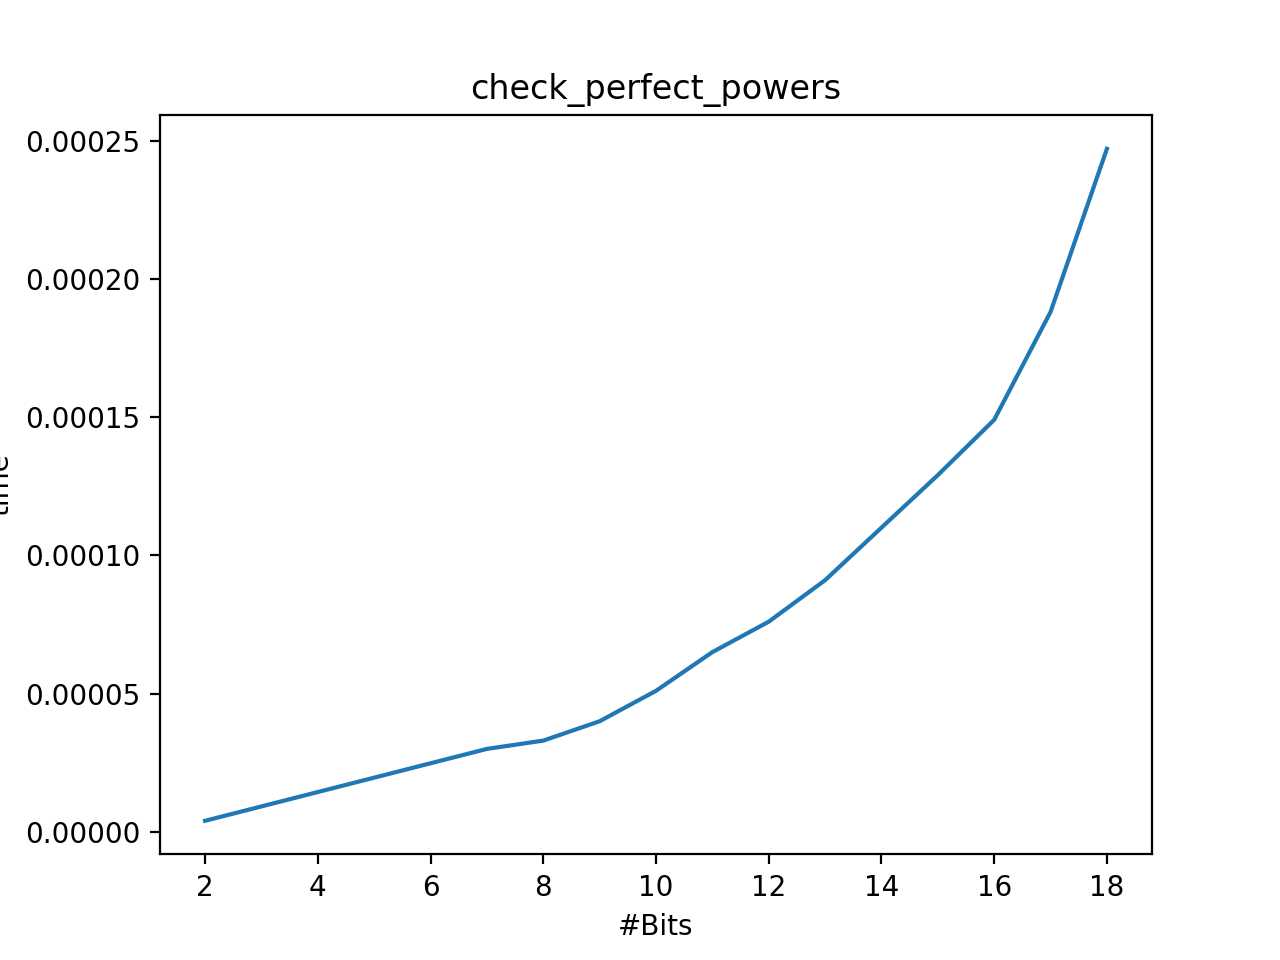
\includegraphics[width=8cm]{plots/pp.png}
\centering
\caption{Laufzeit des Potenz-Prüfung Algorithmus}
\end{figure}

\textbf{Schritt 2:}\newline
Im zweiten Schritt wird ein $r$ gesucht, sodass $o_{r}(n) > log^2 n$. Dies kann durch Ausprobieren von sukzessiven Werten von $r$ und dann zu testen, ob $n^k \neq 1 \,  mod \, r, \, \forall k \leq log^2 n$. Für jedes $r$ gibt es höchstens $O(log^2 n)$ mögliche Werte für $k$. Dies kann in $O^{\sim}(\lVert k \rVert \cdot \rVert r \lVert) = O^{\sim}(log^2 n \, log \, r)$ berechnet werden.\newline\newline
Aus Lemma \ref{limit_of_r} gilt, dass $ r \leq log^5 n$, folglich gilt $O^{\sim}(log^2 n \, log^5 n)$, somit gilt, dass die Laufzeit für den zweiten Schritt $O^{\sim}(log^7 n)$ ist. 


\section{Zusammenfassung}


%%%%%%%%%%%%%%%%%%%%%%%%%%%%
%% Literaturverzeichnis wird 
%% automatisch eingefügt
%%%%%%%%%%%%%%%%%%%%%%%%%%%%
\clearpage
\lhead{}
\printbibliography
\addcontentsline{toc}{section}{\bibname}


%%%%%%%%%%%%%%%%%%%%%%%%%%%%
%% Anhang (optional) 
%%%%%%%%%%%%%%%%%%%%%%%%%%%%
\clearpage
\appendix
\section{Anhang A}

\begin{algorithm}[H]
\SetAlgoLined
\KwIn{$n \in \mathbb{N}, n \geq 2$.}
\begin{enumerate}
\item $a, \, b, \, c, \, m$

\item $ b = 2$.

\item \textbf{while} $2^b \leq n$ \textbf{repeat}

\item $\: \: \: \: $ $a = 1, \, c = n $

\item $\: \: \: \: $ \textbf{while} $c - a \geq 2$ \textbf{repeat}

\item $\: \: \: \: \: \: \: \: \:$ $ m = \lfloor (a + c)/2 \rfloor$

\item $\: \: \: \: \: \: \: \: \:$ $ p = min\{m^b,n+1\}$

\item $\: \: \: \: \: \: \: \: \:$ \textbf{if} $ p = n$ \textbf{return} True.

\item $\: \: \: \: \: \: \: \: \:$ \textbf{if} $p < n$

\item $\: \: \: \: \: \: \: \: \: \: \: \: \: \:$  $ a = m$

\item $\: \: \: \: \: \: \: \: \:$ \textbf{else}

\item $\: \: \: \: \: \: \: \: \: \: \: \: \: \:$  $c = m$

\item $\: \: \: \: $ $b = b + 1$

\item \textbf{return} False


\end{enumerate}
 
\caption{Potenz-Prüfung}
\end{algorithm}

%%%%%%%%%%%%%%%%%%%%%%%%%%%%
%% Eidesstattliche Erklärung
%% muss angepasst werden 
%% in Erklaerung.tex
%%%%%%%%%%%%%%%%%%%%%%%%%%%%
\newpage
\begin{otherlanguage}{ngerman}
\thispagestyle{empty}
\section*{Eidesstattliche Erklärung}
\thispagestyle{empty}
Hiermit versichere ich, die vorliegende Arbeit selbstständig verfasst und keine anderen als die angegebenen Quellen und Hilfsmittel benutzt sowie die Zitate deutlich kenntlich gemacht zu haben.
\newline
\vspace{4\baselineskip}\\
Leipzig, den \today \hfill Salman Salman 
\vspace{4\baselineskip}\\
\end{otherlanguage}

\end{document}
